\documentclass{article}
\usepackage{graphicx} % Required for inserting images
\usepackage[a4paper, total={6in, 8in}]{geometry}
\usepackage{float}

\title{Pattern 1 - Map}
\date{ }

\begin{document}

\maketitle

    One simple parallel pattern is \textbf{map}.  
\begin{figure}[H]
    \centering
    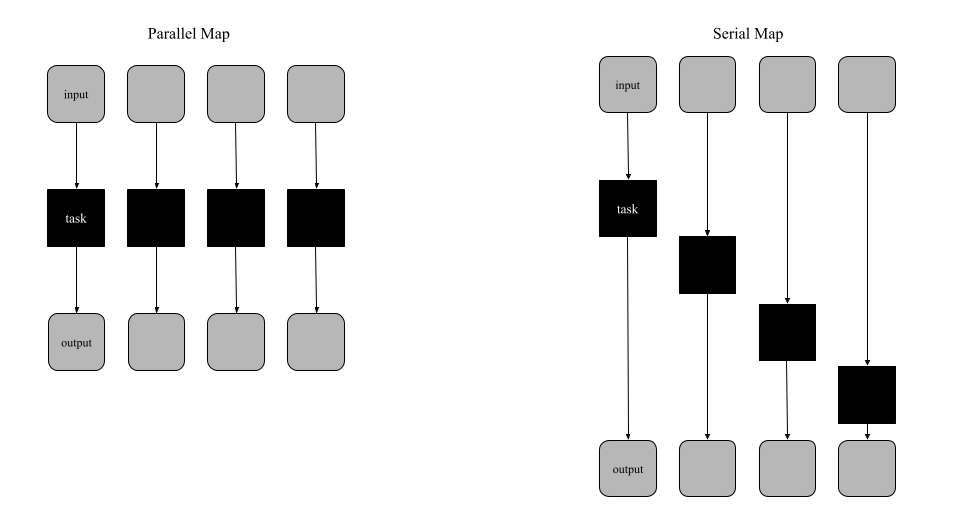
\includegraphics[width=1\linewidth]{Map Diagram.png}
\end{figure}
    In \textbf{map}, there exists two components: a \textbf{collection} of elements and an \textbf{elemental function}. Map runs instances of the elemental function (a task) on each element of the collection. In the world of serial programming, this is synonymous to a for loop in which every iteration is independent of other iterations. Thus, the elemental function should be pure in that it does not modify global data that its instances rely on. If this purity is maintained, map is deterministic (its output should always be the same whenever it is run). \\
    
    Below is a list of topics where maps are often used to improve performance. 
\begin{itemize}
  \item Scaled Vector Addition (SAXPY)
  \item Mandelbrot Set
  \item Gamma Correction
  \item Image Thresholding
  \item Color Space Conversions
  \item Monte Carlo Sampling
  \item Ray Tracing \\
\end{itemize}

    Furthermore, if one has many map patterns occurring in sequence, combining the elemental functions into just one map should be considered! This process, called \textbf{code fusion}, improves performance. 
    
\begin{figure}[H]
    \centering
    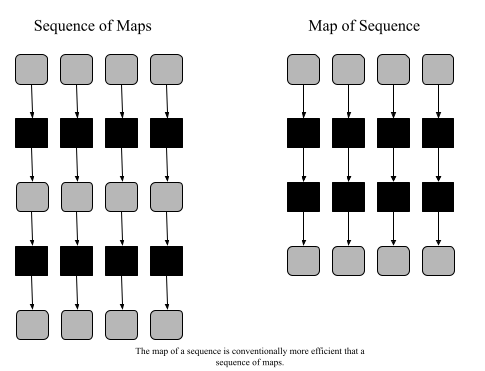
\includegraphics[width=0.75\linewidth]{Sequence of Maps Versus Map of Sequence.png}
\end{figure}


    
\end{document}
